\documentclass[11pt,a4paper]{article}
\usepackage[utf8]{inputenc}
\usepackage[T1]{fontenc}
\usepackage[spanish]{babel}
\usepackage{amsmath, amssymb, amsfonts}
\usepackage{graphicx}
\usepackage{geometry}
\geometry{a4paper, margin=2.5cm}
\usepackage{hyperref}
\hypersetup{
    colorlinks=true,
    linkcolor=blue,
    filecolor=magenta,
    urlcolor=cyan,
}
\usepackage{listings}
\usepackage{caption}
\usepackage{subcaption}
\usepackage{siunitx}
\usepackage{physics} % Para notación física

\title{Informe Parte B2: Integración de $e^{-x^2}$ por Monte Carlo}
\author{Física Computacional II - Isabel Nieto y Camilo Huertas}
\date{\today}

\begin{document}
\maketitle
\tableofcontents
\newpage

\section{Introducción}
El objetivo de esta parte del proyecto es calcular la integral definida de la función $f(x) = e^{-x^2}$ en el intervalo $[0, 1]$ utilizando el método de Monte Carlo por muestreo simple. Se analizará la convergencia del valor estimado de la integral y su error asociado en función del número de muestras $N$ utilizadas en la simulación.

La investigación teórica más amplia sobre el método de Monte Carlo y sus aplicaciones en física estadística se encuentra en el documento principal del proyecto.

\section{Fundamento Teórico}

\subsection{Integración por Monte Carlo (Muestreo Simple)}
Dada una integral unidimensional de la forma:
\begin{equation}
    I = \int_a^b f(x) dx
\end{equation}
Podemos reescribirla como el producto del rango de integración y el valor esperado de $f(x)$ si $x$ es una variable aleatoria uniformemente distribuida en $[a,b]$:
\begin{equation}
    I = (b-a) \int_a^b f(x) p(x) dx = (b-a) \expval{f(X)}
\end{equation}
donde $p(x) = \frac{1}{b-a}$ para $x \in [a,b]$ y $0$ en otro caso.

El método de Monte Carlo estima este valor esperado promediando la función evaluada en $N$ puntos aleatorios $x_i$, generados uniformemente en $[a,b]$:
\begin{equation}
    I_N = (b-a) \frac{1}{N} \sum_{i=1}^N f(x_i)
\end{equation}
Por el Teorema del Límite Central, para $N$ grande, $I_N$ se aproxima a $I$.

\subsection{Estimación del Error}
El error estadístico (error estándar de la media) de la estimación $I_N$ está dado por:
\begin{equation}
    \text{Err}(I_N) = (b-a) \frac{\sigma_f}{\sqrt{N}}
\end{equation}
donde $\sigma_f^2$ es la varianza de la función $f(x)$ en el intervalo $[a,b]$:
\begin{equation}
    \sigma_f^2 = \expval{f^2(X)} - (\expval{f(X)})^2
\end{equation}

En la práctica, estimamos $\expval{f^2(X)}$ y $\expval{f(X)}$ a partir de las muestras:
\begin{align}
    \expval{f(X)} &\approx \frac{1}{N} \sum_{i=1}^N f(x_i) = \overline{f} \\
    \expval{f^2(X)} &\approx \frac{1}{N} \sum_{i=1}^N f^2(x_i) = \overline{f^2}
\end{align}

Entonces, el error estimado es:
\begin{equation}
    \text{Err}(I_N) \approx (b-a) \sqrt{\frac{\overline{f^2} - (\overline{f})^2}{N}}
\end{equation}
Este error disminuye como $N^{-1/2}$.

\subsection{La Integral Específica}
La integral a calcular es $I = \displaystyle\int_0^1 e^{-x^2}\,dx$.

Este valor es $\frac{\sqrt{\pi}}{2}\text{erf}(1)$, donde $\text{erf}(z) = \frac{2}{\sqrt{\pi}}\int_0^z e^{-t^2}dt$ es la función error.

El valor numérico de referencia es aproximadamente $0.7468241328$.

\section{Implementación Computacional}

\subsection{Arquitectura de Software}
Se desarrolló una clase \texttt{IntegradorMonteCarlo} en C++ que implementa el método de muestreo simple:

\begin{itemize}
    \item El constructor recibe la función a integrar (como \texttt{std::function<double(double)>}), los límites de integración y una semilla para el generador de números aleatorios (\texttt{std::mt19937}).
    \item El método \texttt{CalcularIntegralSimple} toma el número de muestras $N$ y devuelve el valor estimado de la integral y el error estándar calculado.
\end{itemize}

\subsection{Programa Principal}
El programa principal (\texttt{main\_montecarlo\_integral.cpp}) utiliza esta clase para:
\begin{itemize}
    \item Calcular la integral de $e^{-x^2}$ para un rango de valores de $N$ (desde $10^1$ hasta $10^7$)
    \item Guardar los resultados (N, valor estimado, error estimado, valor teórico, diferencia absoluta) en el archivo \texttt{integral\_error\_Nmax\_1e7.dat}
    \item Facilitar el análisis posterior y la graficación
\end{itemize}

\section{Resultados y Análisis}

\subsection{Convergencia del Valor de la Integral}
La Figura \ref{fig:integral_valor} muestra el valor estimado de la integral en función del número de muestras $N$.

\begin{figure}[h!]
    \centering
    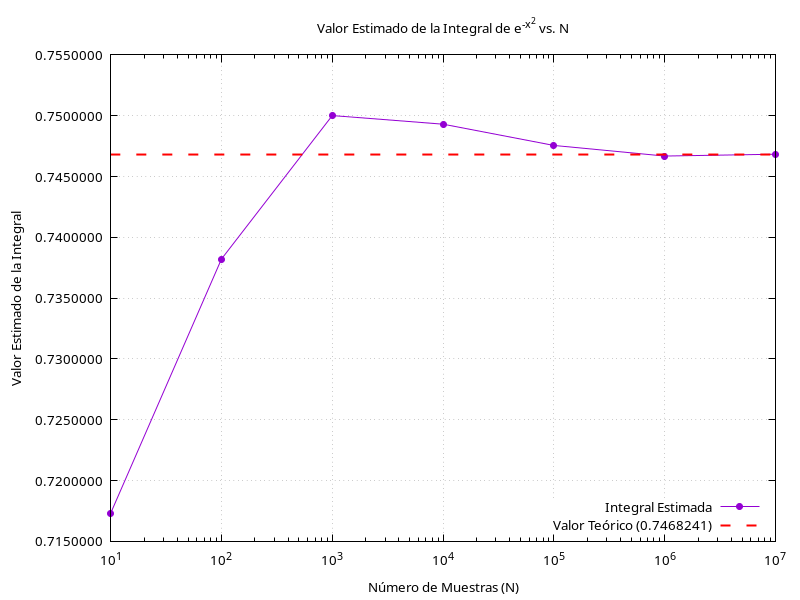
\includegraphics[width=0.8\textwidth]{../results/integral_mc_exp_neg_x2_valor_vs_N.png}
    \caption{Valor estimado de $\int_0^1 e^{-x^2}dx$ en función del número de muestras $N$. La línea roja representa el valor teórico ($\approx 0.7468$).}
    \label{fig:integral_valor}
\end{figure}

El gráfico demuestra que el valor estimado converge al valor teórico a medida que $N$ aumenta, con fluctuaciones estadísticas que disminuyen progresivamente.

\subsection{Convergencia del Error Estimado}
La Figura \ref{fig:integral_error} presenta el error estimado de la integral en función de $N$ en escala log-log.

\begin{figure}[h!]
    \centering
    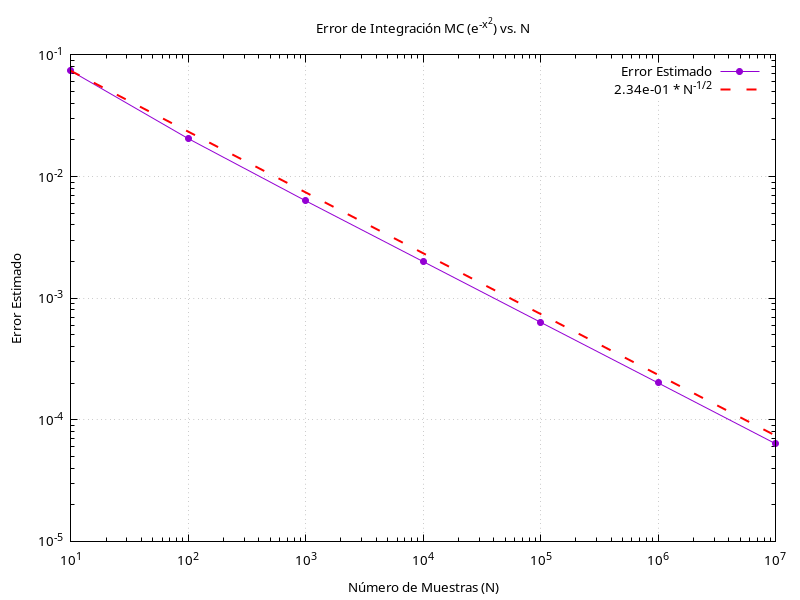
\includegraphics[width=0.8\textwidth]{../results/integral_mc_exp_neg_x2_error_vs_N.png}
    \caption{Error estimado de la integral en función del número de muestras $N$ (escala log-log). La línea roja punteada muestra una referencia con pendiente $N^{-1/2}$.}
    \label{fig:integral_error}
\end{figure}

El análisis log-log confirma la dependencia teórica $N^{-1/2}$ del error, característica fundamental del método de Monte Carlo por muestreo simple.

\subsection{Diferencia Absoluta con el Valor Teórico}
La Figura \ref{fig:integral_diff_abs} analiza la diferencia absoluta entre el valor estimado y el valor teórico.

\begin{figure}[h!]
    \centering
    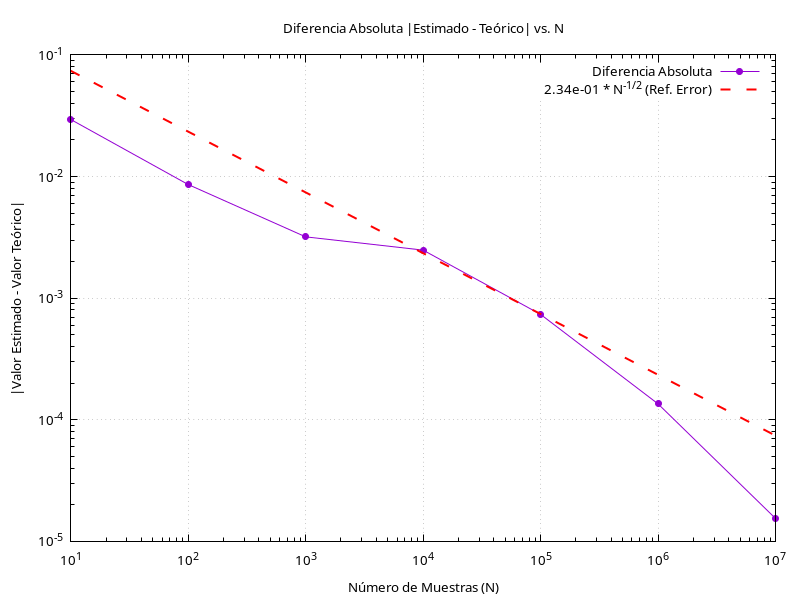
\includegraphics[width=0.8\textwidth]{../results/integral_mc_exp_neg_x2_diff_abs_vs_N.png}
    \caption{Diferencia absoluta $|I_{estimado} - I_{teórico}|$ en función del número de muestras $N$ (escala log-log). La línea roja punteada es la referencia $N^{-1/2}$ del error estimado.}
    \label{fig:integral_diff_abs}
\end{figure}

La diferencia absoluta sigue la tendencia general del error estimado, aunque presenta fluctuaciones estadísticas naturales del proceso estocástico.

\section{Archivos Generados}

El programa genera automáticamente:
\begin{itemize}
    \item \texttt{integral\_error\_Nmax\_1e7.dat}: Datos de convergencia completos
    \item Gráficas PNG generadas por el script \texttt{plot\_integral\_error.gp}
    \item Documentación HTML y LaTeX mediante Doxygen
\end{itemize}

\section{Validación y Verificación}

\subsection{Precisión Numérica}
\begin{itemize}
    \item Uso de \texttt{std::erf} de la biblioteca estándar para el valor de referencia
    \item Precisión de punto flotante de doble precisión para todos los cálculos
    \item Verificación de convergencia para $N = 10^7$ muestras
\end{itemize}

\subsection{Reproducibilidad}
\begin{itemize}
    \item Semilla configurable para el generador Mersenne Twister
    \item Resultados consistentes entre ejecuciones con la misma semilla
    \item Documentación completa del flujo de trabajo
\end{itemize}

\section{Conclusiones}

\subsection{Logros Técnicos}
\begin{enumerate}
    \item Se implementó exitosamente el método de Monte Carlo por muestreo simple
    \item La clase \texttt{IntegradorMonteCarlo} es reutilizable para otras integrales
    \item El flujo de trabajo automatizado facilita la reproducibilidad
    \item La documentación con Doxygen mejora la mantenibilidad del código
\end{enumerate}

\subsection{Resultados Físicos}
\begin{enumerate}
    \item El método converge correctamente al valor teórico de la integral
    \item El error estadístico sigue la ley $N^{-1/2}$ característica de Monte Carlo
    \item Las fluctuaciones observadas son consistentes con la naturaleza estocástica del método
    \item La precisión alcanzada es adecuada para aplicaciones prácticas
\end{enumerate}

\subsection{Relevancia Computacional}
Este trabajo demuestra:
\begin{itemize}
    \item La efectividad del método de Monte Carlo para integración numérica
    \item La importancia del análisis estadístico en métodos estocásticos
    \item El valor de la programación orientada a objetos para simulaciones científicas
    \item La utilidad de herramientas automatizadas para análisis de convergencia
\end{itemize}

\subsection{Aplicaciones y Extensiones}
El código desarrollado puede extenderse para:
\begin{itemize}
    \item Integrales multidimensionales donde métodos deterministas fallan
    \item Técnicas avanzadas como muestreo por importancia
    \item Integración de funciones con singularidades
    \item Aplicaciones en física estadística y mecánica cuántica
\end{itemize}

La implementación proporciona una base sólida para estudios más avanzados en métodos de Monte Carlo y computación científica.

\end{document}
